\documentclass[t]{beamer}

\usepackage[utf8]{inputenc}
\usepackage[T1]{fontenc}
\usepackage{helvet}
\usepackage[english]{babel}

\usetheme{LUH}


% format numbers
\usepackage{siunitx}
%https://tex.cloud.uni-hannover.de/project/6677e7bc8f12321099572893
\sisetup{
  locale=US,
  group-digits = integer,
  round-mode = places,
  round-precision = 3,
  round-pad = false,
  mode = match % the numbers are printed in text or math mode matching their surrounding
}
% better itemize and enumerate
\usepackage{enumitem}
\setlist[itemize]{nosep, label=-} 
% \setlist[enumerate,1]{label=\alph*)}
% enables \enquote command for better quotation
\usepackage[nolist,nohyperlinks]{acronym}
\usepackage{csquotes}
\usepackage{booktabs}

\usepackage{tikz}
\usetikzlibrary{arrows, shapes, positioning, calc}

\usepackage[
  backend=biber,
  natbib=true,
  citestyle=authoryear,
  maxcitenames=1,
  maxbibnames=5,
]{biblatex}
\bibliography{literature.bib}
\renewcommand*{\bibfont}{\normalfont\scriptsize}

\usepackage{hyperref}
\hypersetup{
  pdftitle={Developing Interpretable Style Vectors to Steer Large Language Models towards Group-Specific Explanation Generation},
  pdfsubject={Master's Thesis Presentation},
  pdfauthor={Janek Prange}
  plainpages=false,           %   -
  colorlinks=false,           %   - colorize links?
  pdfborder={0 0 0},          %   -
  breaklinks=true,            %   - allow line break inside links
  bookmarksnumbered=true,     %
  bookmarksopen=true,          %
  pdfpagemode=UseNone,
}

\title[Master's Thesis Presentation]{Developing Interpretable Style Vectors to Steer Large Language Models towards Group-Specific Explanation Generation}
\date{08.04.2025}
% \date[08.04.2025]{08.04.2025}
\author[Prange]{Janek Prange}
\unilogo{
\includegraphics[height=\LUHLogoHeight]{img/luh-logo.png}}
\logo{
\includegraphics[height=\LUHLogoHeight]{img/luh_ai-logo.png}}
\titleimage{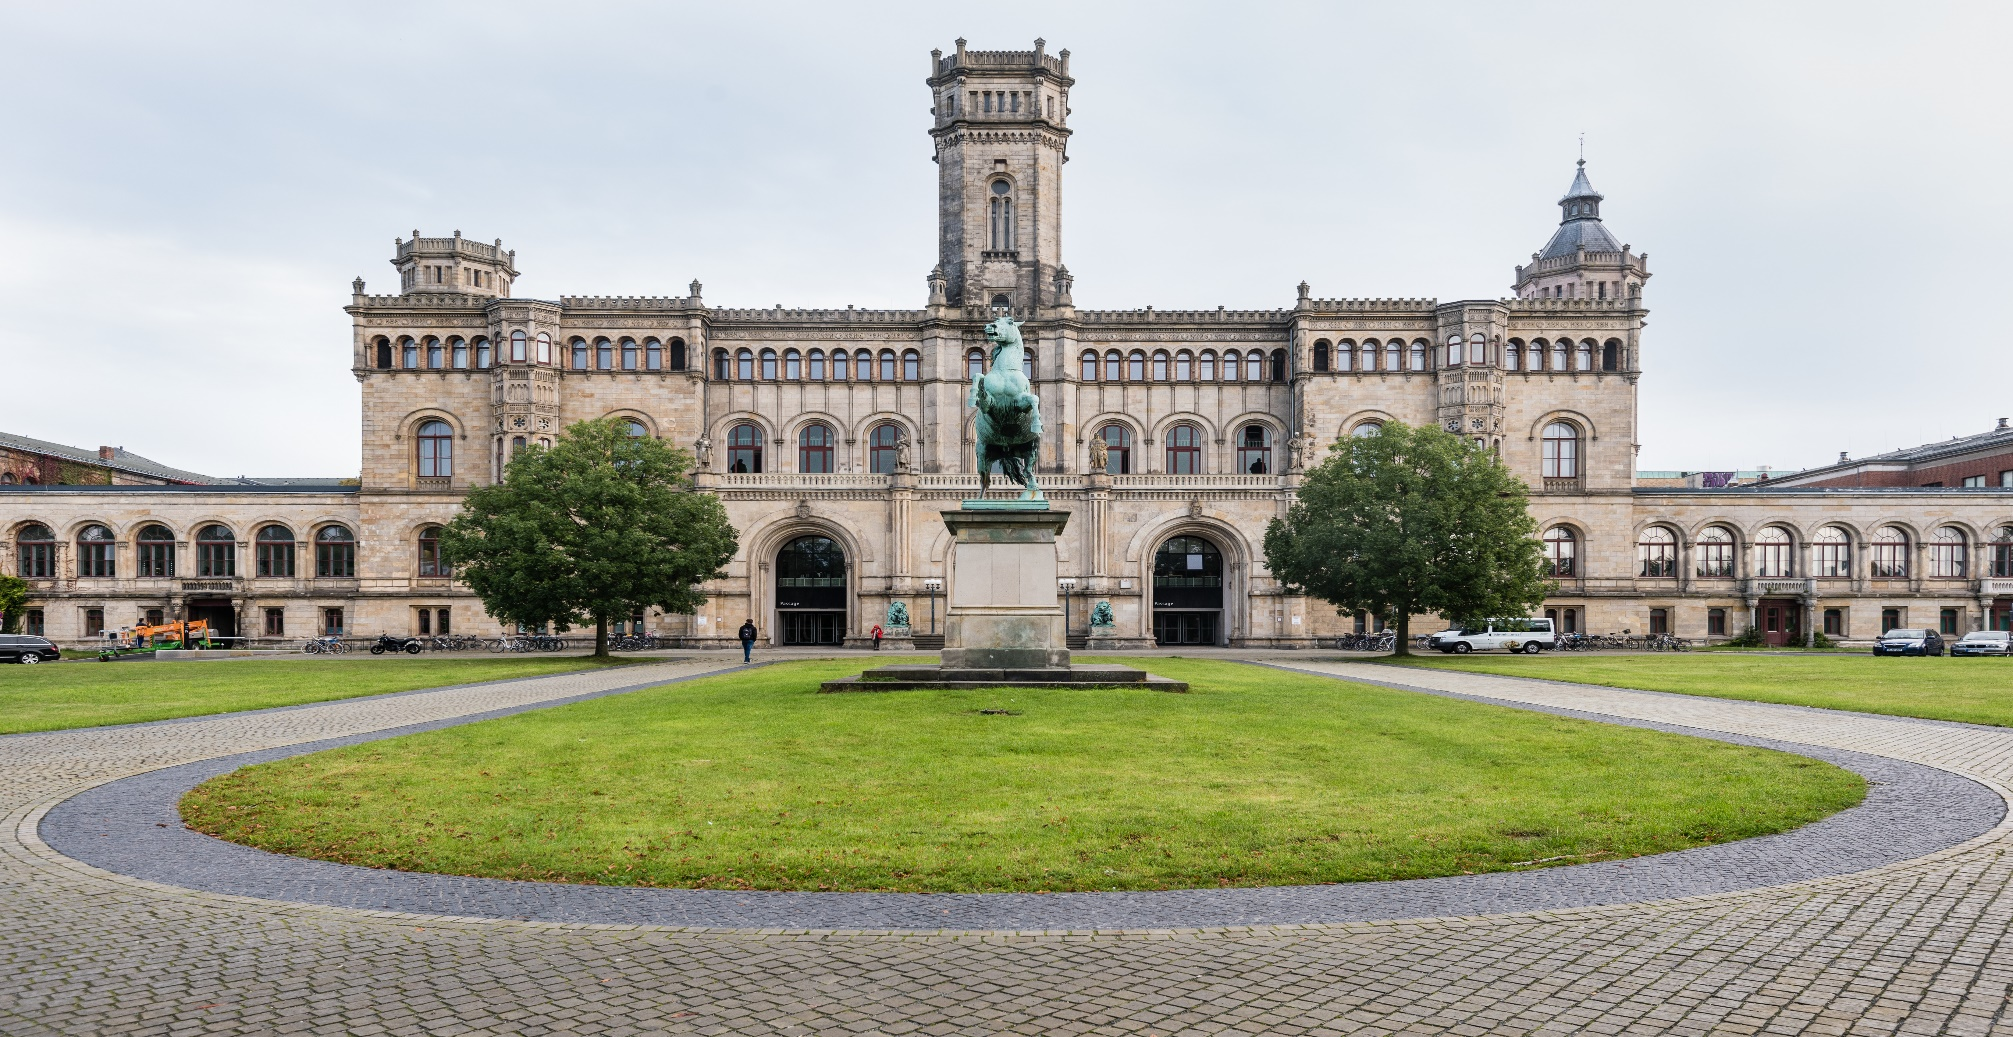
\includegraphics[width=.7\paperwidth]{img/welfenschloss.jpg}}

\newcommand{\footauthorcite}[1]{%
  \footnote{%
    \hangindent=2em % Adjust indentation for proper alignment
    \foreach \x in {#1} {%
        \citeauthor{\x} (\citeyear{\x}), \emph{\citetitle{\x}};
    }
  }%
}

\begin{document}

\begin{frame}
  \titlepage
\end{frame}

\begin{frame}[shrink,t]{Table of Contents}
  \tableofcontents
\end{frame}

\AtBeginSection[]
{
  \begin{frame}[shrink,t]{Table of Contents}
    \tableofcontents[currentsection]
  \end{frame}
}

%%%%%%%%%%%%%%%%%%%%%%%%%%%%%%%%%%%%%%%%%%
\section{Motivation}
% an knowledge attributes denken!
\begin{frame}{Interpretable Style Embeddings}
  \begin{itemize}
    \item
  \end{itemize}
\end{frame}

\begin{frame}{Group-Specific Explanations}
  \begin{itemize}
    \item test\footauthorcite{patelLearningInterpretableStyle2023}
  \end{itemize}
\end{frame}


%%%%%%%%%%%%%%%%%%%%%%%%%%%%%%%%%%%%%%%%%%
\section{Data Collection}
\begin{frame}{Group-Specific Texts}
  \begin{itemize}
    \item Stackex Data
          \begin{itemize}
            \item taken from stackex forums such as % TODO
            \item \num{5500} answers to create the style vector attributes and train SFAM
            \item \num{66000} answers to train LISA
          \end{itemize}
    \item Askx Data
          \begin{itemize}
            \item taken from % TODO
            \item % TODO: how many?
          \end{itemize}
  \end{itemize}
\end{frame}

\begin{frame}{Steering questions}
  \begin{itemize}
    \item 100 questions taken from previous works from \citet{petroni-etal-2021-kilt,rooeinKnowYourAudience2023}
  \end{itemize}
\end{frame}


%%%%%%%%%%%%%%%%%%%%%%%%%%%%%%%%%%%%%%%%%%
% or Creation of the synthetic dataset?
\section{Creation of the Style Vector Attributes}
\subsection{Style Sentence Generation}
\begin{frame}{Style Sentence Generation}
  \begin{itemize}
    \item
  \end{itemize}
\end{frame}

\begin{frame}[shrink]
  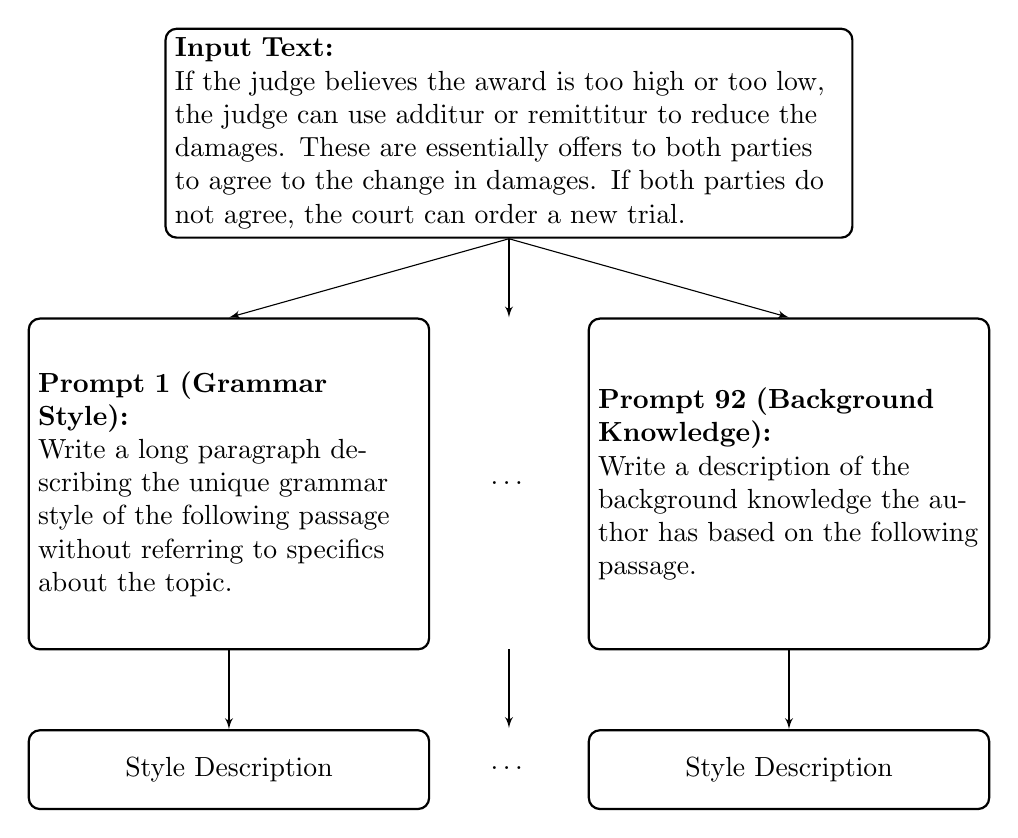
\begin{tikzpicture}
  [> = latex', auto,
    block/.style ={
        rectangle,
        draw=black,
        thick,
        % align=flush center,
        rounded corners,
        % minimum height=4em,
      },
  ]
  \node[block, text width=0.7\linewidth] (answer) {\textbf{Input Text:}\\If the judge believes the award is too high or too low, the judge can use additur or remittitur to reduce the damages. These are essentially offers to both parties to agree to the change in damages. If both parties do not agree, the court can order a new trial.};

  \node[block, minimum height=4.2cm, text width=0.4\linewidth, below left=of answer.south] (prompt1) {\textbf{Prompt 1 (Grammar Style):}\\Write a long paragraph describing the unique grammar style of the following passage without referring to specifics about the topic.};
  \node[align=flush center, minimum height=4.2cm, text width=0.2\linewidth, below=1cm of answer.south] (prompt2) {\ldots};
  \node[block, minimum height=4.2cm, text width=0.4\linewidth, below right=of answer.south] (prompt3) {\textbf{Prompt 92 (Background Knowledge):}\\Write a description of the background knowledge the author has based on the following passage.};

  \draw[->] (answer.south) -- (prompt1.north);
  \draw[->] (answer.south) -- (prompt2.north);
  \draw[->] (answer.south) -- (prompt3.north);

  \node[block, align=flush center, minimum height=1cm, text width=0.4\linewidth, below=1cm of prompt1] (description1) {Style Description};
  \node[align=flush center, minimum height=1cm, text width=0.2\linewidth, below=1cm of prompt2] (description2) {\ldots};
  \node[block, align=flush center, minimum height=1cm, text width=0.4\linewidth, below=1cm of prompt3] (description3) {Style Description};

  \draw[->] (prompt1.south) -- (description1.north);
  \draw[->] (prompt2.south) -- (description2.north);
  \draw[->] (prompt3.south) -- (description3.north);
\end{tikzpicture}

\end{frame}
\begin{frame}[shrink]
  \begin{tikzpicture}
  [> = latex', auto,
    block/.style ={
        rectangle,
        draw=black,
        thick,
        % align=flush center,
        rounded corners,
        % minimum height=4em
      },
  ]
  \node[block, align=flush center, minimum height=1cm, text width=0.4\linewidth, below=1cm of prompt1] (description1) {Style Description};
  \node[align=flush center, minimum height=1cm, text width=0.2\linewidth, below=1cm of prompt2] (description2) {\ldots};
  \node[block, align=flush center, minimum height=1cm, text width=0.4\linewidth, below=1cm of prompt3] (description3) {Style Description};

  \node[block, text width=0.95\linewidth, below=1cm of description2] (sentence_prompt) {\textbf{Prompt:}\\Rewrite this description as a long list of short sentences describing the author's writing style  where each sentence is in the format of \enquote{The author is X.} or \enquote{The author uses X.}.};

  \draw[->] (description1.south) -- ++(0,-1cm);
  \draw[->] (description2.south) -- ++(0,-1cm);
  \draw[->] (description3.south) -- ++(0,-1cm);

  \node[block, text width=0.95\linewidth, below=1cm of sentence_prompt] (attributes) {\textbf{Style Attributes:}\\
    % The author uses the passive voice. \\
    % The author uses active voice. \\
    % The author uses sentence fragments. \\
    % The author uses run-on sentences. \\
    % The author uses words related to visual perception. \\
    % The author uses words expressing wellness. \\
    % The author uses a neutral tone. \\
    The author uses words related to risk. \\
    The author uses words related to allure. \\
    The author uses words indicating poverty. \\
    The author uses words expressing needs. \\
    The author uses numbers. \\
    The author explains legal concepts. \\
    The author uses words indicating men. \\
    The author uses the word judge. \\
    \ldots
  };

  \draw[->] (sentence_prompt.south) -- +(0,-1cm);
  \draw[->] let \p1 = (sentence_prompt.south), \p2 = (description1) in (\x2,\y1) -- +(0,-1cm);
  \draw[->] let \p1 = (sentence_prompt.south), \p2 = (description3) in (\x2,\y1) -- +(0,-1cm);
\end{tikzpicture}

\end{frame}

\subsection{Clustering and Cluster Selection}
\begin{frame}{}

\end{frame}

\begin{frame}{Resulting synthetic dataset}

  \begin{tabular}{lS}
    \toprule
                 & {Number of data points} \\ \midrule
    Answers      & 5500                    \\
    Descriptions &                         \\
    Sentences    &                         \\
    Clusters     &                         \\ \bottomrule
  \end{tabular}

\end{frame}


%%%%%%%%%%%%%%%%%%%%%%%%%%%%%%%%%%%%%%%%%%
\section{Custom Models}
\subsection{SFAM}

\subsection{LISA}

\subsection{Embedding Model}


%%%%%%%%%%%%%%%%%%%%%%%%%%%%%%%%%%%%%%%%%%
\section{Steering Text Generation}
\subsection{Steering with Prompt Engineering}

\subsection{Activation Steering}


%%%%%%%%%%%%%%%%%%%%%%%%%%%%%%%%%%%%%%%%%%
\section{Conclusion}



%%%%%%%%%%%%%%%%%%%%[%%%%%%%%%%%%%%%%%%%%%%
\begin{frame}[c]
  \centering \Large
  Thank you for your attention
\end{frame}


\section*{References}
\begin{frame}[allowframebreaks]{References}
  \printbibliography
\end{frame}


\end{document}
